\documentclass[12pt]{beamer}
\usepackage{booktabs}
\usepackage{tikz}
\usepackage{listings}
\usepackage{color}

\definecolor{mygreen}{rgb}{0,0.6,0}
\definecolor{mygray}{rgb}{0.5,0.5,0.5}
\definecolor{mymauve}{rgb}{0.58,0,0.82}

\lstset{ %
	backgroundcolor=\color{white},   % choose the background color; you must add \usepackage{color} or \usepackage{xcolor}
	basicstyle=\footnotesize,        % the size of the fonts that are used for the code
	breakatwhitespace=false,         % sets if automatic breaks should only happen at whitespace
	breaklines=true,                 % sets automatic line breaking
	captionpos=b,                    % sets the caption-position to bottom
	commentstyle=\color{mygreen},    % comment style
	deletekeywords={...},            % if you want to delete keywords from the given language
	escapeinside={\%*}{*)},          % if you want to add LaTeX within your code
	extendedchars=true,              % lets you use non-ASCII characters; for 8-bits encodings only, does not work with UTF-8
	frame=single,	                   % adds a frame around the code
	keepspaces=true,                 % keeps spaces in text, useful for keeping indentation of code (possibly needs columns=flexible)
	keywordstyle=\color{blue},       % keyword style
	language=C++,                 % the language of the code
	otherkeywords={*,...},           % if you want to add more keywords to the set
	numbers=left,                    % where to put the line-numbers; possible values are (none, left, right)
	numbersep=5pt,                   % how far the line-numbers are from the code
	numberstyle=\tiny\color{mygray}, % the style that is used for the line-numbers
	rulecolor=\color{black},         % if not set, the frame-color may be changed on line-breaks within not-black text (e.g. comments (green here))
	showspaces=false,                % show spaces everywhere adding particular underscores; it overrides 'showstringspaces'
	showstringspaces=false,          % underline spaces within strings only
	showtabs=false,                  % show tabs within strings adding particular underscores
	stepnumber=1,                    % the step between two line-numbers. If it's 1, each line will be numbered
	stringstyle=\color{mymauve},     % string literal style
	tabsize=2,	                   % sets default tabsize to 2 spaces
	title=\lstname                   % show the filename of files included with \lstinputlisting; also try caption instead of title
}
\beamertemplatenavigationsymbolsempty
\AtBeginSection[]
{
    \begin{frame}
    \frametitle{Table of Contents}
    \tableofcontents[currentsection]
    \end{frame}
}

\title{Minimum spanning tree}
\subtitle{Algorithms and variant}
\author{beOI Training}
\institute{
\includegraphics[height=12em]{../share/beoi-logo}}

\begin{document}

\frame{\titlepage}

\section{Definition}

\begin{frame}
\frametitle{Motivating problem}
\begin{center}
	Several neighbourhoods:\\~\\
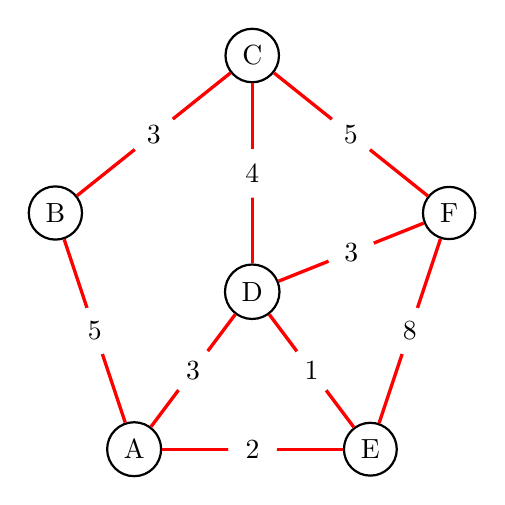
\begin{tikzpicture}
\begin{scope}[every node/.style={circle,thick,draw}]
\node (A) at (1,0) {A};
\node (B) at (0,3) {B};
\node (C) at (2.5,5) {C};
\node (D) at (2.5,2) {D};
\node (E) at (4,0) {E};
\node (F) at (5,3) {F} ;
\end{scope}

\begin{scope}[>={[black]},
every node/.style={fill=white,circle},
every edge/.style={draw=red,very thick}]
\path [->] (A) edge node {$5$} (B);
\path [->] (B) edge node {$3$} (C);
\path [->] (A) edge node {$3$} (D);
\path [->] (D) edge node {$4$} (C);
\path [->] (A) edge node {$2$} (E);
\path [->] (D) edge node {$1$} (E);
\path [->] (D) edge node {$3$} (F);
\path [->] (C) edge node {$5$} (F);
\path [->] (E) edge node {$8$} (F);
\end{scope}
\end{tikzpicture}
\\Connect all of them in the least total weight
\end{center}
\end{frame}

\begin{frame}
\frametitle{Spanning tree}
A tree connecting all nodes in a graph.\\
Tree: no cycles.\\
A graph can have multiple spanning trees.\\~\\
\pause
If a graph has $v$ nodes, how many edges do all its spanning trees have?\\
\pause
\textit{Answer: $v-1$}

\end{frame}

\begin{frame}
\frametitle{Minimum spanning tree}
A spanning tree with the minimum total weight.\\
\pause

\includegraphics[width=0.4\linewidth]{img/captain-obvious}
\pause
\\There can be several minimum spanning trees (mst).\\
Total weight is unique (minimum).

\end{frame}

\section{Kruskal's algorithm}

\begin{frame}
\frametitle{The algorithm}
\begin{enumerate}
	\item Sort al the edges in non-decreasing order of their weight
	\item Pick the smallest edge\\
	Does adding it form a cycle in the ST?
	\begin{itemize}
		\item No:  include it
		\item Yes: discard it
	\end{itemize}
	\item Repeat until ...
	\pause
	the tree contains $v - 1$ edges
\end{enumerate}
\end{frame}

\begin{frame}
	\frametitle{Example}
	Network:\\
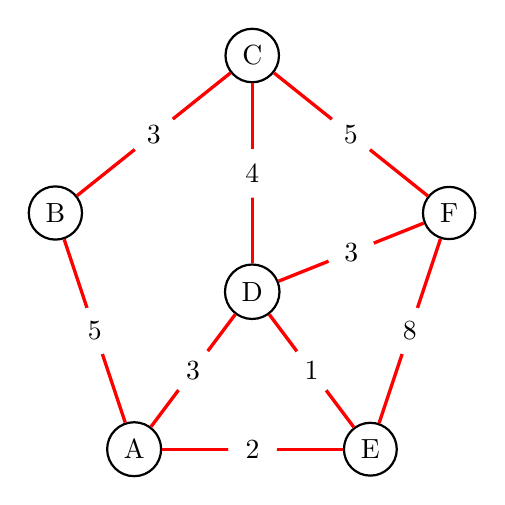
\begin{tikzpicture}
\begin{scope}[every node/.style={circle,thick,draw}]
\node (A) at (1,0) {A};
\node (B) at (0,3) {B};
\node (C) at (2.5,5) {C};
\node (D) at (2.5,2) {D};
\node (E) at (4,0) {E};
\node (F) at (5,3) {F} ;
\end{scope}

\begin{scope}[>={[black]},
every node/.style={fill=white,circle},
every edge/.style={draw=red,very thick}]
\path [->] (A) edge node {$5$} (B);
\path [->] (B) edge node {$3$} (C);
\path [->] (A) edge node {$3$} (D);
\path [->] (D) edge node {$4$} (C);
\path [->] (A) edge node {$2$} (E);
\path [->] (D) edge node {$1$} (E);
\path [->] (D) edge node {$3$} (F);
\path [->] (C) edge node {$5$} (F);
\path [->] (E) edge node {$8$} (F);
\end{scope}
\end{tikzpicture}
\end{frame}

\begin{frame}
	\frametitle{Example}
	Network:\\
	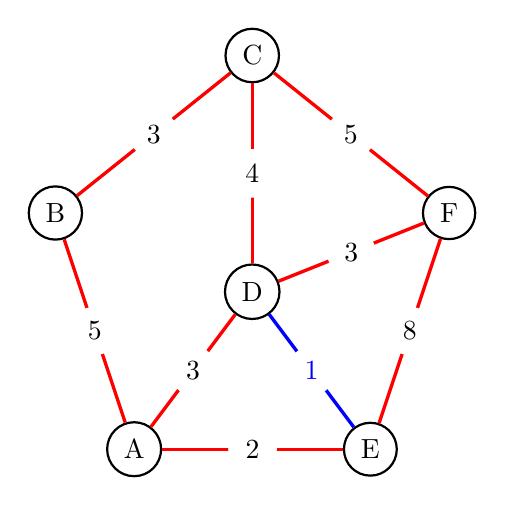
\begin{tikzpicture}
	\begin{scope}[every node/.style={circle,thick,draw}]
	\node (A) at (1,0) {A};
	\node (B) at (0,3) {B};
	\node (C) at (2.5,5) {C};
	\node (D) at (2.5,2) {D};
	\node (E) at (4,0) {E};
	\node (F) at (5,3) {F} ;
	\end{scope}
	
	\begin{scope}[>={[black]},
	every node/.style={fill=white,circle},
	every edge/.style={draw=red,very thick}]
	\path [->] (A) edge node {$5$} (B);
	\path [->] (B) edge node {$3$} (C);
	\path [->] (A) edge node {$3$} (D);
	\path [->] (D) edge node {$4$} (C);
	\path [->] (A) edge node {$2$} (E);
	\path [->] (D) edge[blue] node {$1$} (E);
	\path [->] (D) edge node {$3$} (F);
	\path [->] (C) edge node {$5$} (F);
	\path [->] (E) edge node {$8$} (F);
	\end{scope}
	\end{tikzpicture}
\end{frame}

\begin{frame}
	\frametitle{Example}
	Network:\\
	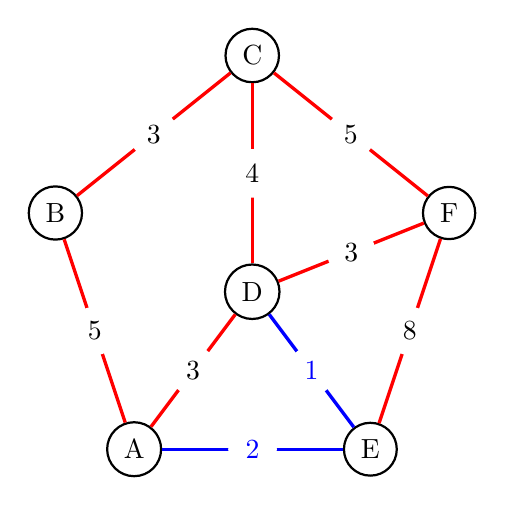
\begin{tikzpicture}
	\begin{scope}[every node/.style={circle,thick,draw}]
	\node (A) at (1,0) {A};
	\node (B) at (0,3) {B};
	\node (C) at (2.5,5) {C};
	\node (D) at (2.5,2) {D};
	\node (E) at (4,0) {E};
	\node (F) at (5,3) {F} ;
	\end{scope}
	
	\begin{scope}[>={[black]},
	every node/.style={fill=white,circle},
	every edge/.style={draw=red,very thick}]
	\path [->] (A) edge node {$5$} (B);
	\path [->] (B) edge node {$3$} (C);
	\path [->] (A) edge node {$3$} (D);
	\path [->] (D) edge node {$4$} (C);
	\path [->] (A) edge[blue] node {$2$} (E);
	\path [->] (D) edge[blue] node {$1$} (E);
	\path [->] (D) edge node {$3$} (F);
	\path [->] (C) edge node {$5$} (F);
	\path [->] (E) edge node {$8$} (F);
	\end{scope}
	\end{tikzpicture}
\end{frame}

\begin{frame}
	\frametitle{Example}
	Network:\\
	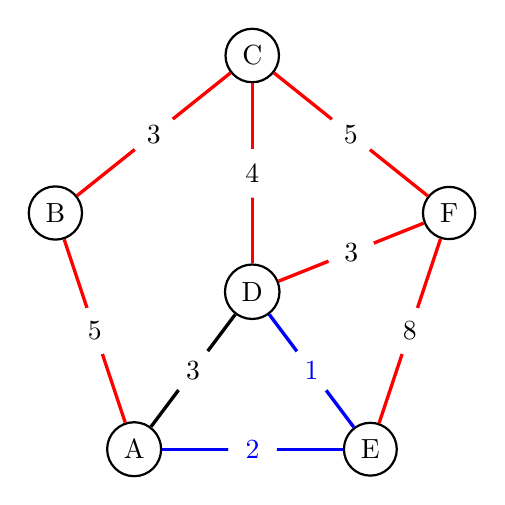
\begin{tikzpicture}
	\begin{scope}[every node/.style={circle,thick,draw}]
	\node (A) at (1,0) {A};
	\node (B) at (0,3) {B};
	\node (C) at (2.5,5) {C};
	\node (D) at (2.5,2) {D};
	\node (E) at (4,0) {E};
	\node (F) at (5,3) {F} ;
	\end{scope}
	
	\begin{scope}[>={[black]},
	every node/.style={fill=white,circle},
	every edge/.style={draw=red,very thick}]
	\path [->] (A) edge node {$5$} (B);
	\path [->] (B) edge node {$3$} (C);
	\path [->] (A) edge[black] node {$3$} (D);
	\path [->] (D) edge node {$4$} (C);
	\path [->] (A) edge[blue] node {$2$} (E);
	\path [->] (D) edge[blue] node {$1$} (E);
	\path [->] (D) edge node {$3$} (F);
	\path [->] (C) edge node {$5$} (F);
	\path [->] (E) edge node {$8$} (F);
	\end{scope}
	\end{tikzpicture}
\end{frame}

\begin{frame}
	\frametitle{Example}
	Network:\\
	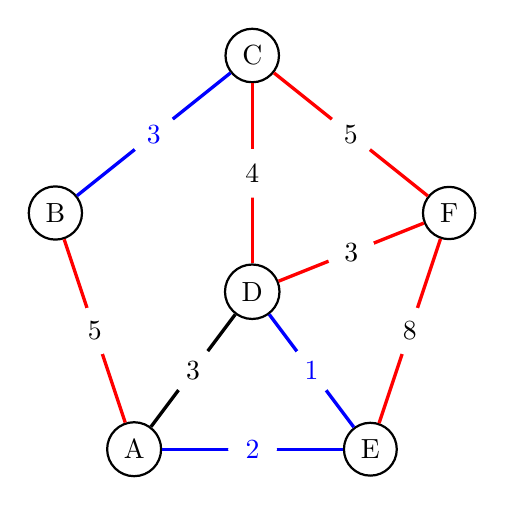
\begin{tikzpicture}
	\begin{scope}[every node/.style={circle,thick,draw}]
	\node (A) at (1,0) {A};
	\node (B) at (0,3) {B};
	\node (C) at (2.5,5) {C};
	\node (D) at (2.5,2) {D};
	\node (E) at (4,0) {E};
	\node (F) at (5,3) {F} ;
	\end{scope}
	
	\begin{scope}[>={[black]},
	every node/.style={fill=white,circle},
	every edge/.style={draw=red,very thick}]
	\path [->] (A) edge node {$5$} (B);
	\path [->] (B) edge[blue] node {$3$} (C);
	\path [->] (A) edge[black] node {$3$} (D);
	\path [->] (D) edge node {$4$} (C);
	\path [->] (A) edge[blue] node {$2$} (E);
	\path [->] (D) edge[blue] node {$1$} (E);
	\path [->] (D) edge node {$3$} (F);
	\path [->] (C) edge node {$5$} (F);
	\path [->] (E) edge node {$8$} (F);
	\end{scope}
	\end{tikzpicture}
\end{frame}
\begin{frame}
	\frametitle{Example}
	Network:\\
	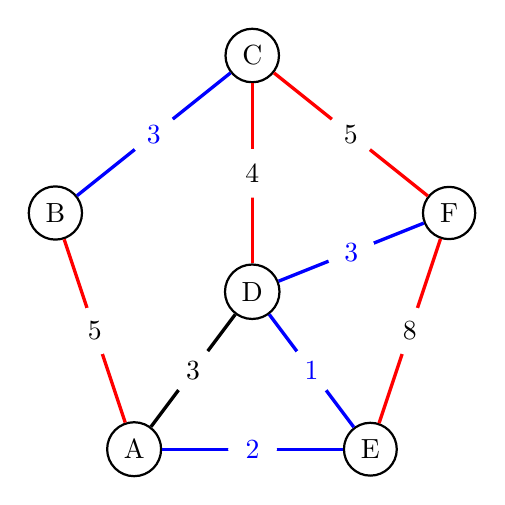
\begin{tikzpicture}
	\begin{scope}[every node/.style={circle,thick,draw}]
	\node (A) at (1,0) {A};
	\node (B) at (0,3) {B};
	\node (C) at (2.5,5) {C};
	\node (D) at (2.5,2) {D};
	\node (E) at (4,0) {E};
	\node (F) at (5,3) {F} ;
	\end{scope}
	
	\begin{scope}[>={[black]},
	every node/.style={fill=white,circle},
	every edge/.style={draw=red,very thick}]
	\path [->] (A) edge node {$5$} (B);
	\path [->] (B) edge[blue] node {$3$} (C);
	\path [->] (A) edge[black] node {$3$} (D);
	\path [->] (D) edge node {$4$} (C);
	\path [->] (A) edge[blue] node {$2$} (E);
	\path [->] (D) edge[blue] node {$1$} (E);
	\path [->] (D) edge[blue] node {$3$} (F);
	\path [->] (C) edge node {$5$} (F);
	\path [->] (E) edge node {$8$} (F);
	\end{scope}
	\end{tikzpicture}
\end{frame}

\begin{frame}
	\frametitle{Example}
	Network:\\
	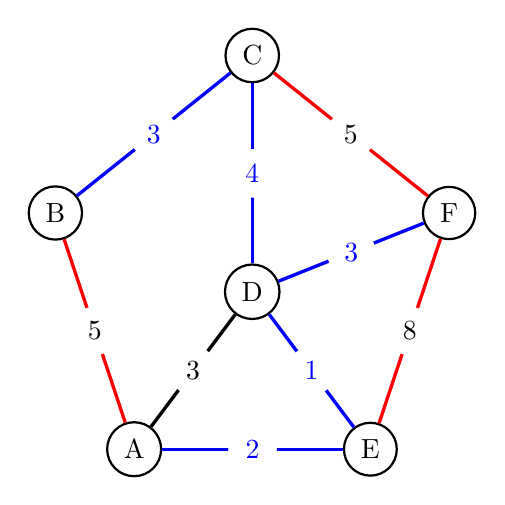
\begin{tikzpicture}
	\begin{scope}[every node/.style={circle,thick,draw}]
	\node (A) at (1,0) {A};
	\node (B) at (0,3) {B};
	\node (C) at (2.5,5) {C};
	\node (D) at (2.5,2) {D};
	\node (E) at (4,0) {E};
	\node (F) at (5,3) {F} ;
	\end{scope}
	
	\begin{scope}[>={[black]},
	every node/.style={fill=white,circle},
	every edge/.style={draw=red,very thick}]
	\path [->] (A) edge node {$5$} (B);
	\path [->] (B) edge[blue] node {$3$} (C);
	\path [->] (A) edge[black] node {$3$} (D);
	\path [->] (D) edge[blue] node {$4$} (C);
	\path [->] (A) edge[blue] node {$2$} (E);
	\path [->] (D) edge[blue] node {$1$} (E);
	\path [->] (D) edge[blue] node {$3$} (F);
	\path [->] (C) edge node {$5$} (F);
	\path [->] (E) edge node {$8$} (F);
	\end{scope}
	\end{tikzpicture}
\end{frame}
\begin{frame}
	\frametitle{Example}
	MST:\\
	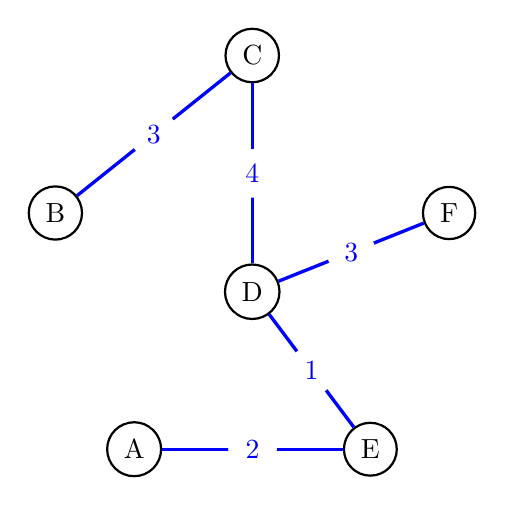
\begin{tikzpicture}
	\begin{scope}[every node/.style={circle,thick,draw}]
	\node (A) at (1,0) {A};
	\node (B) at (0,3) {B};
	\node (C) at (2.5,5) {C};
	\node (D) at (2.5,2) {D};
	\node (E) at (4,0) {E};
	\node (F) at (5,3) {F} ;
	\end{scope}
	
	\begin{scope}[>={[black]},
	every node/.style={fill=white,circle},
	every edge/.style={draw=red,very thick}]
	\path [->] (A) edge[white] node {$5$} (B);
	\path [->] (B) edge[blue] node {$3$} (C);
	\path [->] (A) edge[white] node {$3$} (D);
	\path [->] (D) edge[blue] node {$4$} (C);
	\path [->] (A) edge[blue] node {$2$} (E);
	\path [->] (D) edge[blue] node {$1$} (E);
	\path [->] (D) edge[blue] node {$3$} (F);
	\path [->] (C) edge[white] node {$5$} (F);
	\path [->] (E) edge[white] node {$8$} (F);
	\end{scope}
	\end{tikzpicture}
	\\Cost: 13
\end{frame}
\begin{frame}
	\frametitle{Check for cycles}
	Any ideas?\\
	\pause
	
\includegraphics[width=0.5\linewidth]{img/uf}\\
	\pause
	When you encounter an edge
	\begin{itemize}
		\item check for cycle by finding the parents of source/target vertex
		\item union the two nodes 
	\end{itemize}
	

\end{frame}
\begin{frame}
	\frametitle{Code}
	\lstinputlisting[language=C++,firstline=26,lastline=38]{code/kruskal.cpp}
\end{frame}

\section{Prim's algorithm}

\begin{frame}
	\frametitle{The algorithm}
	\begin{enumerate}
		\item Associate a value for each node
		\begin{itemize}
			\item $0$ for the initial node (arbitrary)
			\item $\infty$ for the rest
		\end{itemize}
		\item Take the node with the smallest value that hasn't been added yet
		\begin{enumerate}
			\item Set the value of all adjacent edges to the minimum of the current value and the edge.
		\end{enumerate}
		\item Repeat \textbf{2} until all nodes have been added
	\end{enumerate}
\end{frame}

\begin{frame}
	\frametitle{Example}
	Network:\\~\\
	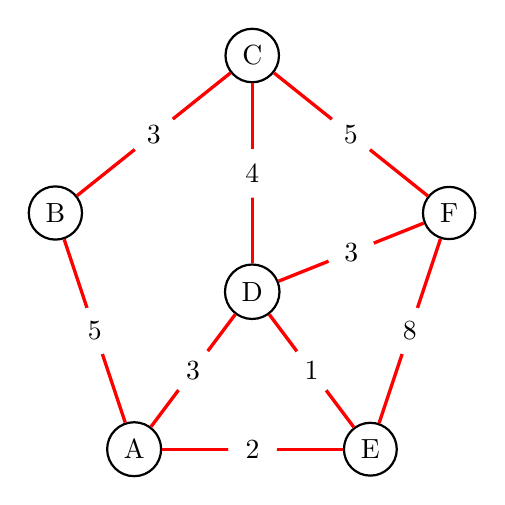
\begin{tikzpicture}
	\begin{scope}[every node/.style={circle,thick,draw}]
	\node (A) at (1,0) {A};
	\node (B) at (0,3) {B};
	\node (C) at (2.5,5) {C};
	\node (D) at (2.5,2) {D};
	\node (E) at (4,0) {E};
	\node (F) at (5,3) {F} ;
	\end{scope}
	
	\begin{scope}[>={[black]},
	every node/.style={fill=white,circle},
	every edge/.style={draw=red,very thick}]
	\path [->] (A) edge node {$5$} (B);
	\path [->] (B) edge node {$3$} (C);
	\path [->] (A) edge node {$3$} (D);
	\path [->] (D) edge node {$4$} (C);
	\path [->] (A) edge node {$2$} (E);
	\path [->] (D) edge node {$1$} (E);
	\path [->] (D) edge node {$3$} (F);
	\path [->] (C) edge node {$5$} (F);
	\path [->] (E) edge node {$8$} (F);
	\end{scope}
	\end{tikzpicture}
\end{frame}
\begin{frame}
	\frametitle{Example}
	Network with values:\\~\\
	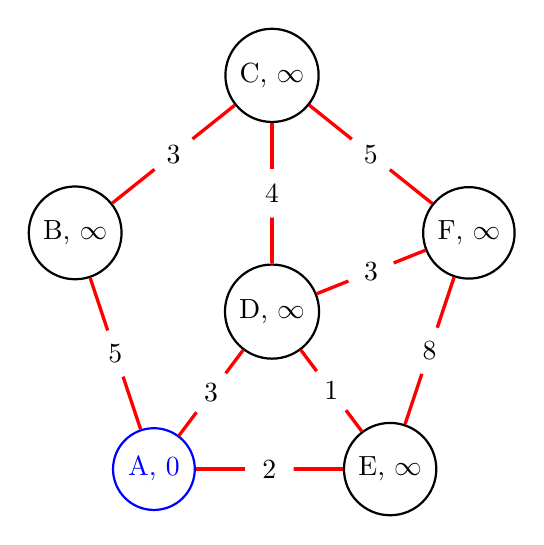
\begin{tikzpicture}
	\begin{scope}[every node/.style={circle,thick,draw}]
	\node[blue] (A) at (1,0) {A, 0};
	\node (B) at (0,3) {B, $\infty$};
	\node (C) at (2.5,5) {C, $\infty$};
	\node (D) at (2.5,2) {D, $\infty$};
	\node (E) at (4,0) {E, $\infty$};
	\node (F) at (5,3) {F, $\infty$} ;
	\end{scope}
	
	\begin{scope}[>={[black]},
	every node/.style={fill=white,circle},
	every edge/.style={draw=red,very thick}]
	\path [->] (A) edge node {$5$} (B);
	\path [->] (B) edge node {$3$} (C);
	\path [->] (A) edge node {$3$} (D);
	\path [->] (D) edge node {$4$} (C);
	\path [->] (A) edge node {$2$} (E);
	\path [->] (D) edge node {$1$} (E);
	\path [->] (D) edge node {$3$} (F);
	\path [->] (C) edge node {$5$} (F);
	\path [->] (E) edge node {$8$} (F);
	\end{scope}
	\end{tikzpicture}
\end{frame}

\begin{frame}
	\frametitle{Example}
	Network with values:\\~\\
	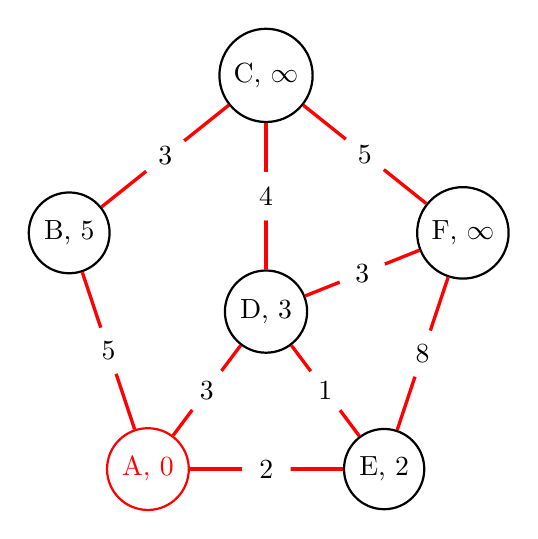
\begin{tikzpicture}
	\begin{scope}[every node/.style={circle,thick,draw}]
	\node[red] (A) at (1,0) {A, 0};
	\node (B) at (0,3) {B, 5};
	\node (C) at (2.5,5) {C, $\infty$};
	\node (D) at (2.5,2) {D, 3};
	\node (E) at (4,0) {E, 2};
	\node (F) at (5,3) {F, $\infty$} ;
	\end{scope}
	
	\begin{scope}[>={[black]},
	every node/.style={fill=white,circle},
	every edge/.style={draw=red,very thick}]
	\path [->] (A) edge node {$5$} (B);
	\path [->] (B) edge node {$3$} (C);
	\path [->] (A) edge node {$3$} (D);
	\path [->] (D) edge node {$4$} (C);
	\path [->] (A) edge node {$2$} (E);
	\path [->] (D) edge node {$1$} (E);
	\path [->] (D) edge node {$3$} (F);
	\path [->] (C) edge node {$5$} (F);
	\path [->] (E) edge node {$8$} (F);
	\end{scope}
	\end{tikzpicture}
\end{frame}

\begin{frame}
	\frametitle{Example}
	Network with values:\\~\\
	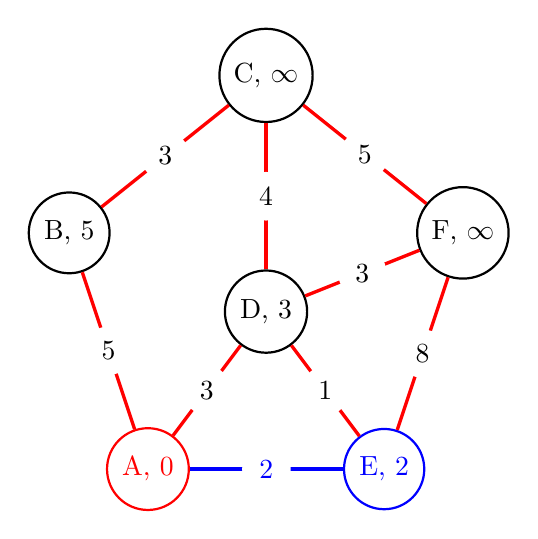
\begin{tikzpicture}
	\begin{scope}[every node/.style={circle,thick,draw}]
	\node[red] (A) at (1,0) {A, 0};
	\node (B) at (0,3) {B, 5};
	\node (C) at (2.5,5) {C, $\infty$};
	\node (D) at (2.5,2) {D, 3};
	\node[blue] (E) at (4,0) {E, 2};
	\node (F) at (5,3) {F, $\infty$} ;
	\end{scope}
	
	\begin{scope}[>={[black]},
	every node/.style={fill=white,circle},
	every edge/.style={draw=red,very thick}]
	\path [->] (A) edge node {$5$} (B);
	\path [->] (B) edge node {$3$} (C);
	\path [->] (A) edge node {$3$} (D);
	\path [->] (D) edge node {$4$} (C);
	\path [->] (A) edge[blue] node {$2$} (E);
	\path [->] (D) edge node {$1$} (E);
	\path [->] (D) edge node {$3$} (F);
	\path [->] (C) edge node {$5$} (F);
	\path [->] (E) edge node {$8$} (F);
	\end{scope}
	\end{tikzpicture}
\end{frame}

\begin{frame}
	\frametitle{Example}
	Network with values:\\~\\
	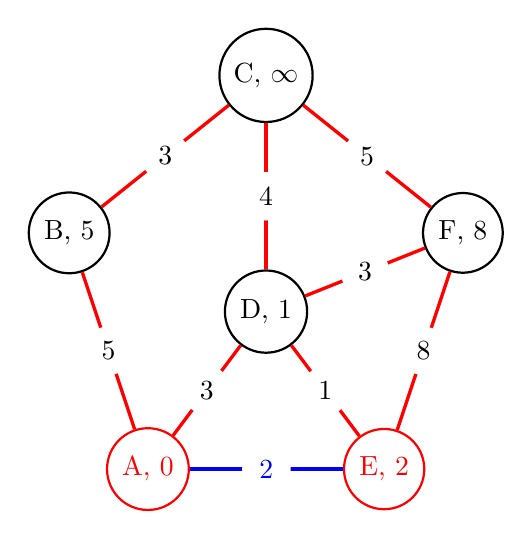
\begin{tikzpicture}
	\begin{scope}[every node/.style={circle,thick,draw}]
	\node[red] (A) at (1,0) {A, 0};
	\node (B) at (0,3) {B, 5};
	\node (C) at (2.5,5) {C, $\infty$};
	\node (D) at (2.5,2) {D, 1};
	\node[red] (E) at (4,0) {E, 2};
	\node (F) at (5,3) {F, 8} ;
	\end{scope}
	
	\begin{scope}[>={[black]},
	every node/.style={fill=white,circle},
	every edge/.style={draw=red,very thick}]
	\path [->] (A) edge node {$5$} (B);
	\path [->] (B) edge node {$3$} (C);
	\path [->] (A) edge node {$3$} (D);
	\path [->] (D) edge node {$4$} (C);
	\path [->] (A) edge[blue] node {$2$} (E);
	\path [->] (D) edge node {$1$} (E);
	\path [->] (D) edge node {$3$} (F);
	\path [->] (C) edge node {$5$} (F);
	\path [->] (E) edge node {$8$} (F);
	\end{scope}
	\end{tikzpicture}
\end{frame}

\begin{frame}
	\frametitle{Example}
	Network with values:\\~\\
	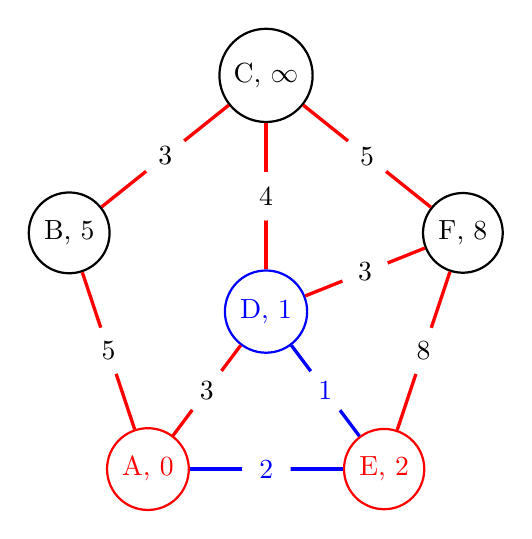
\begin{tikzpicture}
	\begin{scope}[every node/.style={circle,thick,draw}]
	\node[red] (A) at (1,0) {A, 0};
	\node (B) at (0,3) {B, 5};
	\node (C) at (2.5,5) {C, $\infty$};
	\node[blue] (D) at (2.5,2) {D, 1};
	\node[red] (E) at (4,0) {E, 2};
	\node (F) at (5,3) {F, 8} ;
	\end{scope}
	
	\begin{scope}[>={[black]},
	every node/.style={fill=white,circle},
	every edge/.style={draw=red,very thick}]
	\path [->] (A) edge node {$5$} (B);
	\path [->] (B) edge node {$3$} (C);
	\path [->] (A) edge node {$3$} (D);
	\path [->] (D) edge node {$4$} (C);
	\path [->] (A) edge[blue] node {$2$} (E);
	\path [->] (D) edge[blue] node {$1$} (E);
	\path [->] (D) edge node {$3$} (F);
	\path [->] (C) edge node {$5$} (F);
	\path [->] (E) edge node {$8$} (F);
	\end{scope}
	\end{tikzpicture}
\end{frame}

\begin{frame}
	\frametitle{Example}
	Network with values:\\~\\
	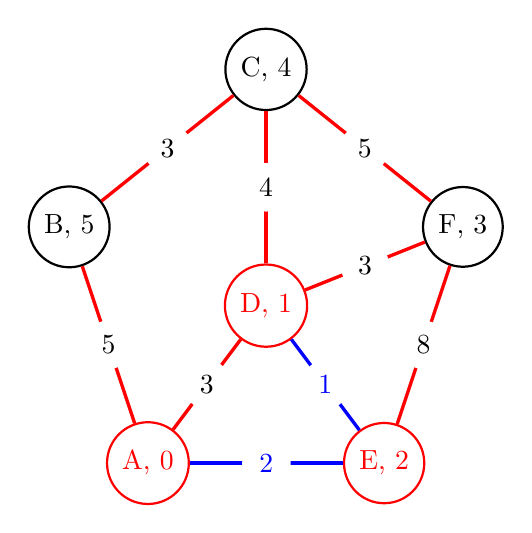
\begin{tikzpicture}
	\begin{scope}[every node/.style={circle,thick,draw}]
	\node[red] (A) at (1,0) {A, 0};
	\node (B) at (0,3) {B, 5};
	\node (C) at (2.5,5) {C, 4};
	\node[red] (D) at (2.5,2) {D, 1};
	\node[red] (E) at (4,0) {E, 2};
	\node (F) at (5,3) {F, 3} ;
	\end{scope}
	
	\begin{scope}[>={[black]},
	every node/.style={fill=white,circle},
	every edge/.style={draw=red,very thick}]
	\path [->] (A) edge node {$5$} (B);
	\path [->] (B) edge node {$3$} (C);
	\path [->] (A) edge node {$3$} (D);
	\path [->] (D) edge node {$4$} (C);
	\path [->] (A) edge[blue] node {$2$} (E);
	\path [->] (D) edge[blue] node {$1$} (E);
	\path [->] (D) edge node {$3$} (F);
	\path [->] (C) edge node {$5$} (F);
	\path [->] (E) edge node {$8$} (F);
	\end{scope}
	\end{tikzpicture}
\end{frame}

\begin{frame}
	\frametitle{Example}
	Network with values:\\~\\
	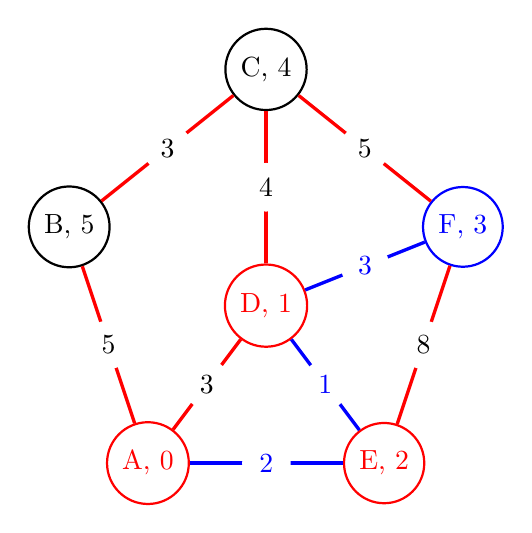
\begin{tikzpicture}
	\begin{scope}[every node/.style={circle,thick,draw}]
	\node[red] (A) at (1,0) {A, 0};
	\node (B) at (0,3) {B, 5};
	\node (C) at (2.5,5) {C, 4};
	\node[red] (D) at (2.5,2) {D, 1};
	\node[red] (E) at (4,0) {E, 2};
	\node[blue] (F) at (5,3) {F, 3} ;
	\end{scope}
	
	\begin{scope}[>={[black]},
	every node/.style={fill=white,circle},
	every edge/.style={draw=red,very thick}]
	\path [->] (A) edge node {$5$} (B);
	\path [->] (B) edge node {$3$} (C);
	\path [->] (A) edge node {$3$} (D);
	\path [->] (D) edge node {$4$} (C);
	\path [->] (A) edge[blue] node {$2$} (E);
	\path [->] (D) edge[blue] node {$1$} (E);
	\path [->] (D) edge[blue] node {$3$} (F);
	\path [->] (C) edge node {$5$} (F);
	\path [->] (E) edge node {$8$} (F);
	\end{scope}
	\end{tikzpicture}
\end{frame}

\begin{frame}
	\frametitle{Example}
	Network with values:\\~\\
	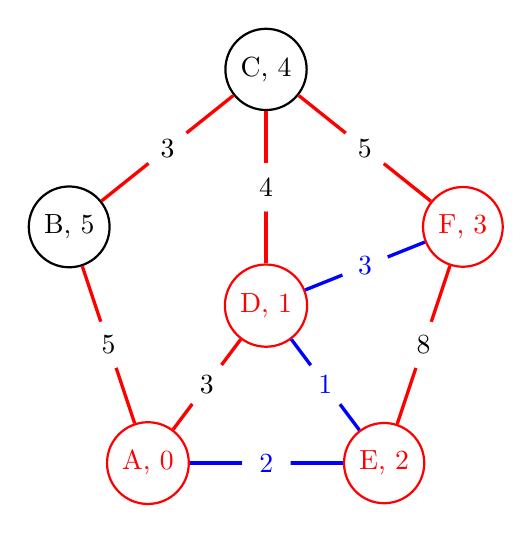
\begin{tikzpicture}
	\begin{scope}[every node/.style={circle,thick,draw}]
	\node[red] (A) at (1,0) {A, 0};
	\node (B) at (0,3) {B, 5};
	\node (C) at (2.5,5) {C, 4};
	\node[red] (D) at (2.5,2) {D, 1};
	\node[red] (E) at (4,0) {E, 2};
	\node[red] (F) at (5,3) {F, 3} ;
	\end{scope}
	
	\begin{scope}[>={[black]},
	every node/.style={fill=white,circle},
	every edge/.style={draw=red,very thick}]
	\path [->] (A) edge node {$5$} (B);
	\path [->] (B) edge node {$3$} (C);
	\path [->] (A) edge node {$3$} (D);
	\path [->] (D) edge node {$4$} (C);
	\path [->] (A) edge[blue] node {$2$} (E);
	\path [->] (D) edge[blue] node {$1$} (E);
	\path [->] (D) edge[blue] node {$3$} (F);
	\path [->] (C) edge node {$5$} (F);
	\path [->] (E) edge node {$8$} (F);
	\end{scope}
	\end{tikzpicture}
\end{frame}

\begin{frame}
	\frametitle{Example}
	Network with values:\\~\\
	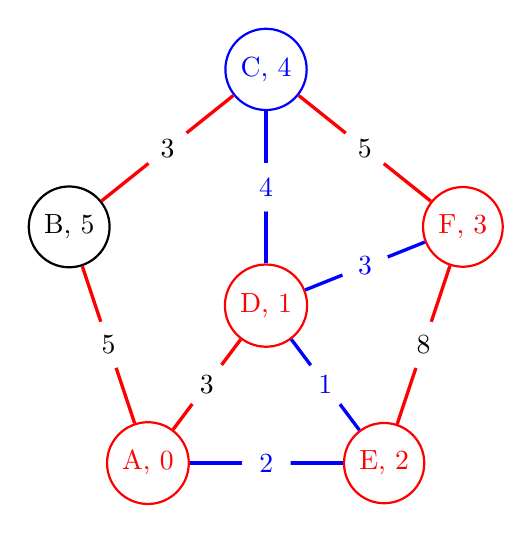
\begin{tikzpicture}
	\begin{scope}[every node/.style={circle,thick,draw}]
	\node[red] (A) at (1,0) {A, 0};
	\node (B) at (0,3) {B, 5};
	\node[blue] (C) at (2.5,5) {C, 4};
	\node[red] (D) at (2.5,2) {D, 1};
	\node[red] (E) at (4,0) {E, 2};
	\node[red] (F) at (5,3) {F, 3} ;
	\end{scope}
	
	\begin{scope}[>={[black]},
	every node/.style={fill=white,circle},
	every edge/.style={draw=red,very thick}]
	\path [->] (A) edge node {$5$} (B);
	\path [->] (B) edge node {$3$} (C);
	\path [->] (A) edge node {$3$} (D);
	\path [->] (D) edge[blue] node {$4$} (C);
	\path [->] (A) edge[blue] node {$2$} (E);
	\path [->] (D) edge[blue] node {$1$} (E);
	\path [->] (D) edge[blue] node {$3$} (F);
	\path [->] (C) edge node {$5$} (F);
	\path [->] (E) edge node {$8$} (F);
	\end{scope}
	\end{tikzpicture}
\end{frame}

\begin{frame}
	\frametitle{Example}
	Network with values:\\~\\
	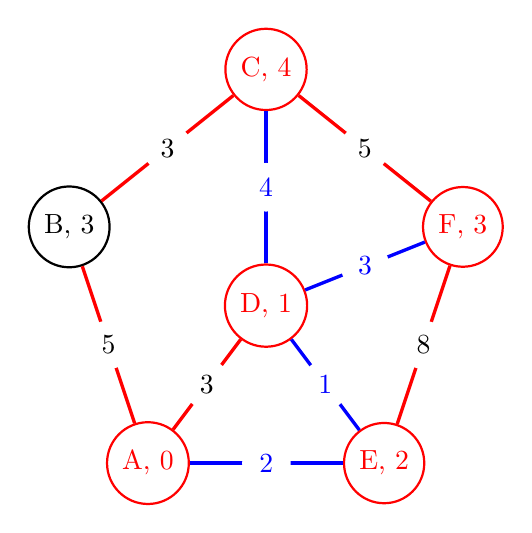
\begin{tikzpicture}
	\begin{scope}[every node/.style={circle,thick,draw}]
	\node[red] (A) at (1,0) {A, 0};
	\node (B) at (0,3) {B, 3};
	\node[red] (C) at (2.5,5) {C, 4};
	\node[red] (D) at (2.5,2) {D, 1};
	\node[red] (E) at (4,0) {E, 2};
	\node[red] (F) at (5,3) {F, 3} ;
	\end{scope}
	
	\begin{scope}[>={[black]},
	every node/.style={fill=white,circle},
	every edge/.style={draw=red,very thick}]
	\path [->] (A) edge node {$5$} (B);
	\path [->] (B) edge node {$3$} (C);
	\path [->] (A) edge node {$3$} (D);
	\path [->] (D) edge[blue] node {$4$} (C);
	\path [->] (A) edge[blue] node {$2$} (E);
	\path [->] (D) edge[blue] node {$1$} (E);
	\path [->] (D) edge[blue] node {$3$} (F);
	\path [->] (C) edge node {$5$} (F);
	\path [->] (E) edge node {$8$} (F);
	\end{scope}
	\end{tikzpicture}
\end{frame}

\begin{frame}
	\frametitle{Example}
	Network with values:\\~\\
	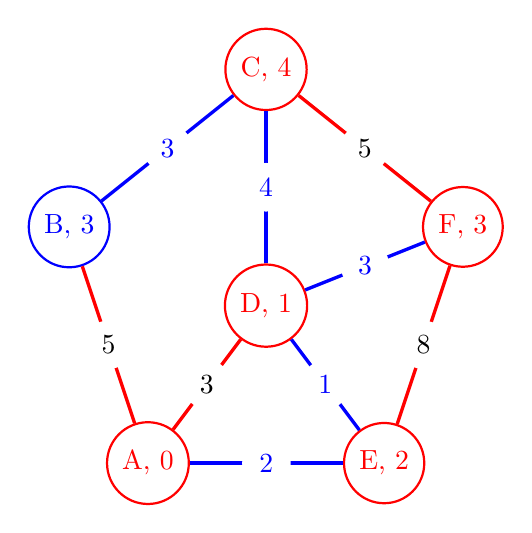
\begin{tikzpicture}
	\begin{scope}[every node/.style={circle,thick,draw}]
	\node[red] (A) at (1,0) {A, 0};
	\node[blue] (B) at (0,3) {B, 3};
	\node[red] (C) at (2.5,5) {C, 4};
	\node[red] (D) at (2.5,2) {D, 1};
	\node[red] (E) at (4,0) {E, 2};
	\node[red] (F) at (5,3) {F, 3} ;
	\end{scope}
	
	\begin{scope}[>={[black]},
	every node/.style={fill=white,circle},
	every edge/.style={draw=red,very thick}]
	\path [->] (A) edge node {$5$} (B);
	\path [->] (B) edge[blue] node {$3$} (C);
	\path [->] (A) edge node {$3$} (D);
	\path [->] (D) edge[blue] node {$4$} (C);
	\path [->] (A) edge[blue] node {$2$} (E);
	\path [->] (D) edge[blue] node {$1$} (E);
	\path [->] (D) edge[blue] node {$3$} (F);
	\path [->] (C) edge node {$5$} (F);
	\path [->] (E) edge node {$8$} (F);
	\end{scope}
	\end{tikzpicture}
\end{frame}

\begin{frame}
	\frametitle{Example}
	MST:\\~\\
	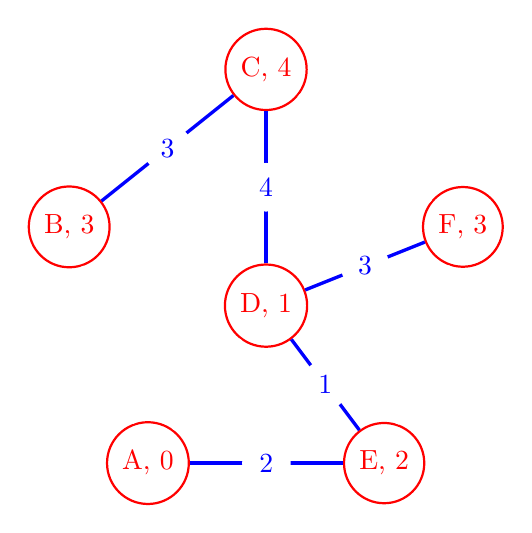
\begin{tikzpicture}
	\begin{scope}[every node/.style={circle,thick,draw}]
	\node[red] (A) at (1,0) {A, 0};
	\node[red] (B) at (0,3) {B, 3};
	\node[red] (C) at (2.5,5) {C, 4};
	\node[red] (D) at (2.5,2) {D, 1};
	\node[red] (E) at (4,0) {E, 2};
	\node[red] (F) at (5,3) {F, 3} ;
	\end{scope}
	
	\begin{scope}[>={[black]},
	every node/.style={fill=white,circle},
	every edge/.style={draw=red,very thick}]
	\path [->] (A) edge[white] node {$5$} (B);
	\path [->] (B) edge[blue] node {$3$} (C);
	\path [->] (A) edge[white] node {$3$} (D);
	\path [->] (D) edge[blue] node {$4$} (C);
	\path [->] (A) edge[blue] node {$2$} (E);
	\path [->] (D) edge[blue] node {$1$} (E);
	\path [->] (D) edge[blue] node {$3$} (F);
	\path [->] (C) edge[white] node {$5$} (F);
	\path [->] (E) edge[white] node {$8$} (F);
	\end{scope}
	\end{tikzpicture}\\
	Cost: 13
\end{frame}

\begin{frame}
	\frametitle{Find minimum}
	Possibilities: 
	\begin{itemize}
		\item Linear search every time: $O(v)$ per node $\rightarrow O(v^2)$
		\item Use a heap (priority queue): $O(vlog(v))$
	\end{itemize}
	\pause
	This algorithm reminds me of someone?\\
	\pause
	This handsome fellow:\\
	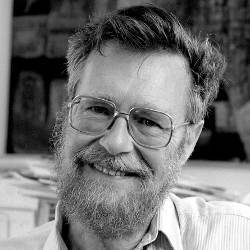
\includegraphics[width=0.4\linewidth]{img/dijkstra.jpg}
	\pause
	\\ Hint: it's Dijkstra
\end{frame}

\begin{frame}
	\frametitle{Code}
	Inside main:\\
	\lstinputlisting[language=C++, firstline=10, lastline=19]{code/prim.cpp}
\end{frame}
\begin{frame}
\frametitle{Code}
Process function:\\
\lstinputlisting[language=C++, firstline=1, lastline=8]{code/prim.cpp}
\end{frame}


\section{Variants}

\begin{frame}
	\frametitle{Maximum spanning tree}
	Spanning tree with maximum total weight.\\~\\
	Any ideas?\\
	\pause
	Solution: 
	\begin{itemize}
		\item Compute the minimum spanning tree with opposite weights
		\item Use kruskal but sort the other way around
	\end{itemize}
	
\end{frame}

\begin{frame}
	\frametitle{'Minimum' spanning subgraph}
	MST where some given edges have to be included in the result.\\~\\
	Any ideas?\\
	\pause
	Solution: First add the necessary edges, then just continue running kruskal on the remaining edges until it's spanning
	
\end{frame}

\begin{frame}
	\frametitle{Minimum 'spanning forest'}
	A spanning forest (multiple trees) of K connected components, with the least total weight.\\~\\
	Any ideas?\\
	\pause
	Solution: Run Kruskal until you have the required number of connected components.
	
\end{frame}

\begin{frame}
	\frametitle{Second best spanning tree}
	Literally what the title says.\\~\\
	Any ideas?\\
	\pause
	Solution: Run Kruskal once to find the MST. For each edge in the MST, compute the MST without using this edge. Find the best of these.
	
\end{frame}

\begin{frame}
	\frametitle{Minimax}
	The minimum of maximum edge weight among all posible paths between two nodes.\\
	Example: find the minimax for 1 and 4\\
	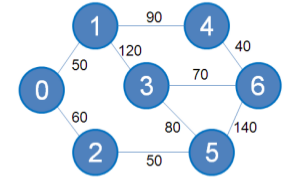
\includegraphics[width=0.6\linewidth]{img/minimax-graph}
\end{frame}

\begin{frame}
	\frametitle{Minimax}
	The minimum of maximum edge weight among all posible paths between two nodes.\\
	Example: find the minimax for 1 and 4\\
	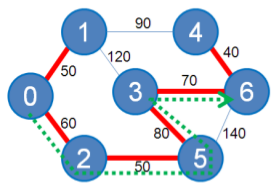
\includegraphics[width=0.6\linewidth]{img/minimax-graph-correct}\\
	The minimax in this case is 80.
\end{frame}

\begin{frame}
	\frametitle{Minimax}
	The minimum of maximum edge weight among all posible paths between two nodes.\\~\\
	How would you solve this?\\
	Solution: Compute the MST and traverse it from source to target.
\end{frame}

\end{document}
